\scanpage{15}
\uline{Exercice}\qquad Réalisation régulière d'un polygône.

Soit $\deleted{V}E$ plan affine euclidien sur $\mathbb{R}$ (avec metrique déf pos. sur \unsure{l'espace|l'esp|l'esp.} $V$ des translations). Une réalisation rectiligne d'un polygone $(S,A,R)$ est dite \uline{régulière} si tous les cotes du polygône ont $=$
% The two-line addition stands to the right of longueur. Its enclosing line is
% open at the left-hand tail; the separate comma remains beside that opening.
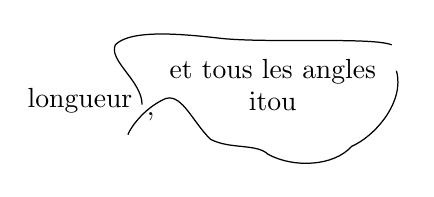
\begin{tikzpicture}[baseline=(longueur.base),x=1cm,y=1cm]
  \node[anchor=base west,inner sep=0pt] (longueur) at (0,0) {longueur};
  \node[anchor=base,inner sep=0pt] at (1.57,-.10) {,};
  \node[anchor=center,inner sep=0pt] at (3.12,.29)
    {\inserted{\shortstack{et tous les angles\\itou}}};
  \draw[line width=.45pt]
    (1.46,.04) .. controls (1.46,.34) and (1.03,.60) .. (1.12,.80)
    .. controls (1.32,1.01) and (2.04,.93) .. (2.48,.88)
    .. controls (3.12,.82) and (4.38,.90) .. (4.63,.80);
  \draw[line width=.45pt]
    (4.69,.47) .. controls (4.80,.08) and (4.42,-.36) .. (4.12,-.49)
    .. controls (3.90,-.74) and (3.39,-.77) .. (3.06,-.59)
    .. controls (2.91,-.45) and (2.58,-.53) .. (2.33,-.40)
    .. controls (2.09,-.17) and (1.95,.23) .. (1.72,.10)
    .. controls (1.48,-.02) and (1.32,-.24) .. (1.28,-.34);
\end{tikzpicture}
\uline{régulière} \deleted{et} \uline{\unsure{normalisee|normalisée}} si la dite longueur est $1$.

a) Existence, grâce à équation cyclotomique $z^n=1$ dans $\mathbb{C}$.

b) Prouver que si $(V\deleted{\unsure{,}}\supset P\deleted{\unsure{,}}\supset\deleted{\unsure{A|B}}S)$ et $(V'\supset P'\supset S')$ sont deux $n$-polygônes ($n\geq3$) munis d'une \unsure{rèal.|réal.} rectiligne \uline{rég.} (resp \unsure{normalisee|normalisée}) il existe une \deleted{\unsure{iso|isom}} similitude (resp \unsure{isom}) \deleted{\uline{unique}} de $V$ sur $V'$, qui transforme $P$ et $P^{\unsure{\prime|!}}$, $S$ en $S'$; \tikz[baseline=(cancel.base),x=1em,y=1em]{
  \node[inner sep=0pt,anchor=base west] (cancel) at (0,0) {\deleted{si $V\unsure{;|,}P,S$}};
  % The cancellation has a separate hooked return at its left end.
  \draw[line width=.4pt] (-.55,.25) .. controls (-.35,-.02) and (.12,-.06) .. (.62,.3);
  \draw[line width=.4pt] (-.55,.25) -- (-.12,.35);
} plus précisément, pour tt isom (comb) de $(\deleted{P}\unsure{S},A,R)$ sur $(S',A',R')$, $\exists\,\unsure{\vert|1}$ similitude
% The addition is above de V. A rising curved arrow runs beneath it and ends
% just above the corrected V; the baseline text remains de V sur V'.
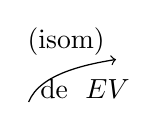
\begin{tikzpicture}[baseline=(de.base),x=1cm,y=1cm]
  \node[anchor=base west,inner sep=0pt] (de) at (.16,0) {de};
  \node[anchor=base,inner sep=0pt] (oldV) at (1.02,0) {$\deleted{\unsure{E}}V$};
  \node[anchor=base west,inner sep=0pt] at (0,.63) {\inserted{(isom)}};
  \draw[->,line width=.45pt] (.02,-.05)
    .. controls (.16,.31) and (.76,.43) .. (1.13,.49);
\end{tikzpicture}
sur $V'$ qui l'induise. \deleted{Montrer que}

\deleted{\unsure{Ex|Cor}}\quad\uline{Cor} Notion d'enveloppe affine (ou vectorielle, grâce : centre de
% The addition is above gravité), with its independent closing parenthesis.
% The curved lead meets short forked strokes and a longer oblique stroke.
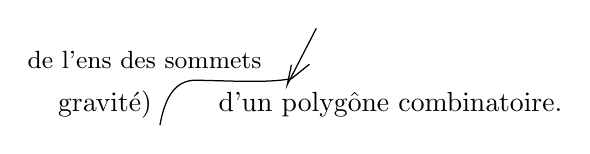
\begin{tikzpicture}[baseline=(gravite.base),x=1em,y=1em]
  \node[anchor=base west,inner sep=0pt] (gravite) at (0,0) {gravité)};
  \node[anchor=base west,inner sep=0pt,font=\small] at (-1.1,1.55)
    {\inserted{de l'ens des sommets}};
  \node[anchor=base west,inner sep=0pt] at (5.8,0) {d'un polygône combinatoire.};
  \draw[line width=.45pt] (3.7,-.5)
    .. controls (3.95,.9) and (4.5,1.18) .. (5.2,1.12)
    .. controls (6.3,1.1) and (7.6,1.02) .. (8.45,1.18);
  \draw[line width=.45pt] (8.45,1.18) -- (9.1,1.70);
  \draw[line width=.45pt] (9.35,3.0) -- (8.30,.96) -- (8.45,1.68);
\end{tikzpicture}

\deleted{\unsure{Si|Soit}} Orientation du polygône $\longleftrightarrow$ orientation de son enveloppe
% Two detached dark points below the right end of the last line: writing versus surface trace remains uncertain.
\par\vspace{2.5\baselineskip}\noindent\hfill
\unsure{\tikz[baseline=-.3ex]{
  \fill (0,0) ellipse (.055em and .035em);
  \fill (.14em,.24em) ellipse (.035em and .055em);
}}\hspace*{2em}\par
% archive sheet number: 14
